\documentclass[a4paper,10pt]{article}

\usepackage[utf8]{inputenc}
\usepackage{mathtools}
\usepackage{amsfonts}
\usepackage{amsmath}


\title{\textbf{Computer Graphics} \\ Final Project}
\author{Thierry CANTENOT \\ J114030901}
\date{23/06/15}

\pdfinfo{%
  /Title    (Final Project)
  /Author   (Thierry CANTENOT)
  /Creator  ()
  /Producer ()
  /Subject  (Computer Graphics)
  /Keywords ()
}

\begin{document}
\maketitle

\begin{figure}[!htb]\centering
    \frame{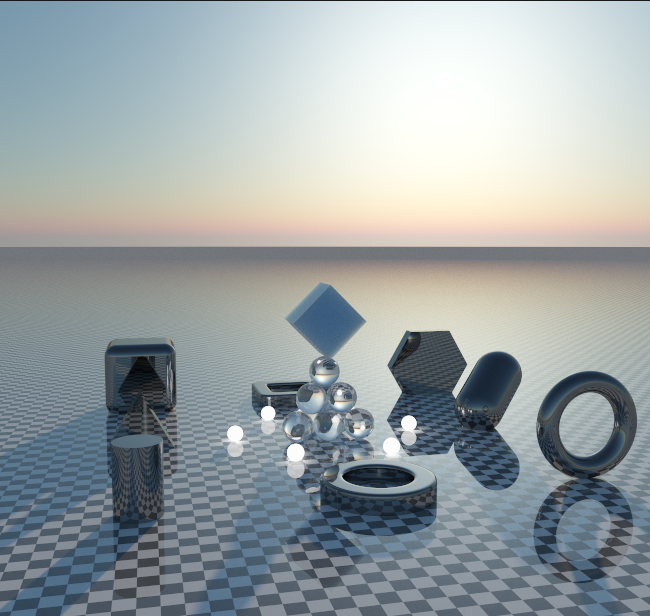
\includegraphics[width=0.9\linewidth]{./images/img1.png}}
\end{figure}


\pagebreak
\section{Introduction}

For the final project, I decided to implement a "real-time" pathtracer in GLSL (OpenGL Shading Language) with Python as front-end. \\
The pathtracer and the scenes are implemented in GLSL, and therefore run directly on the GPU. This allows to get "interactive" framerate for simple scenes. The interactivity is reached before the scene convergence is done by accumulating the radiance frame by frame, one sample per pixel at a time.\\
The camera of the scene is a kind a trackball camera that can be manipulated with the mouse in order to change the point of view.

\section{Features}

\subsection{Pathtracer}


The pathtracer uses Monte-Carlo integration to approximate the rendering equations. The pathtracer allows to use a full Monte-Carlo in order to be able to generate caustics and reflected lights from mirrors; however the convergence of the integration is slow. It also allows to perform \textbf{direct light sampling} to accelerate the convergence at the cost of not being able to generate caustics or reflected light.\\

\noindent
To speed up, the convergence of the image, \textbf{importance sampling} can also be used in the case of diffuse surfaces. Instead of throwing a bouncing ray uniformly on the normal-oriented hemisphere of the surface, I use a cosine-weighted distribution to concentrate the bouncing rays in the direction they would contribute the most to the illumination (greatest cosine factor $N.L$). \\

\noindent
Another technique I used to accelerate convergence is \textbf{stratified sampling}. Instead of drawing random values uniformly over the full range $[0, 1]$, I constraint them to some sub-range and then move to the next sub-range when I draw another random number. This avoid the unlucky cases where the random samples are no well-distributed and are too concentrated in one area. \\

\noindent
\textbf{Termination criterion}\\
In my pathtracer, three criterion can be used to stop the ray "recursion":
\begin{itemize}
	\item The ray depth: set a maximum number of bounces for one ray (50 by default).
	\item The current accumulated reflectance: if the reflectance coefficient becomes too low, the ray is stopped because it will probably not contribute much anymore to the illumination.
	\item The Russian Roulette: unbiased method used in statistics to accelerate the computation of a integral (here the rendering equation)
\end{itemize}


\noindent
I implemented two methods to perform ray intersections: \textbf{ray tracing} and \textbf{ray marching distance fields}.

\subsubsection{Ray tracing}

My pathtracer uses recursive ray tracing to generate the images. In order to use ray tracing to draw a primitive, we must know the analytic formula of intersection between the ray and the primitive.

\subsubsection{Ray marching distance fields}

My pathtracer can also perform ray marching on distance fields. This method is useful when the analytical formula of intersection is not known. To perform ray marching on distance fields, we need a function that returns the distance to the primitive. This distance can be signed (positive when outside the primitive, negative when inside) or unsigned (positive when outside, and 0 inside). Then by "marching" along the ray, i.e by doing some small steps on  the ray, we can get as close as we want to the surface of the primitive. When a minimal distance is reached, we consider that we hit the primitive. I used a method called "\textbf{sphere tracing}" to perform optimal steps during the ray marching procedure. \\

\noindent
In the pathtracer, ray tracing and ray marching are interchangeable because they are both methods used to compute an intersection point. However, the scene representation depends on the method used: analytic formulae for ray tracing and distance fields for ray marching.

\subsection{Illumination models}

Several surface types are supported by the pathtracer:
\begin{itemize}
	\item Pure diffuse (ideal diffuse)
	\item Reflective diffuse (like acrylic)
	\item Metallic
	\item Refractive (glass, \ldots)
	\item Emissive (indirect lights, \ldots)
\end{itemize}

\subsubsection{Phong model}

The standard Phong model is used to compute the diffuse and specular components of the radiance function.

\subsubsection{Reflection \& Refraction}

I am using physically based reflection and refraction in the pathtracer by implementing the Snell's law and the Fresnel's equations. The refractive index of the material is used to perform the reflection and refraction computations.\\

\noindent
Snell's law:
\begin{equation}
	\frac{sin(\theta_i)}{sin(\theta_t)} = \frac{n_2}{n_1}
\end{equation}
where $\theta_i$ and $\theta_t$ are respectively the angle of incidence and the angle of refraction, and $n_1$ and $n_2$ the indices of refraction of the incident medium and of the transmitted medium. \\

\noindent
Fresnel's equations:
\begin{equation}
\left.\begin{aligned}
    R_s &= (\frac{n_1cos(\theta_i) - n_2cos(\theta_t)}{n_1cos(\theta_i) + n_2cos(\theta_t)})^2 \qquad \text{, reflectance for s-polarized light}& \\
    R_p &= (\frac{n_1cos(\theta_t) - n_2cos(\theta_i)}{n_1cos(\theta_t) + n_2cos(\theta_i)})^2 \qquad \text{, reflectance for p-polarized light}& \\
    R   &= \frac{R_s + R_p}{2} \qquad \text{, reflectance}&\\
    T   &= 1 - R \qquad \text{, transmittance}
\end{aligned}\right.
\end{equation}
where $R$ is the reflectance, i.e the fraction of reflected light at the interface between the two media, and $T$ transmittance, i.e the fraction of transmitted light.

\subsubsection{Absorption \& Scattering}

I also implemented absorption and scattering. Each material has an absorption coefficient (3 values for RGB) and a scattering coefficient. \\
The absorption equation is as follow:
\begin{equation}
	T = \exp^{-a \times d}
\end{equation}
where $T$ is the spectral (RGB) transmitted fraction of light, $a$ is the material spectral absoprtion coefficient and $d$ is the distance travelled inside the absorbing medium. \\

\noindent
The scattering equation is as follow:
\begin{equation}
\left.\begin{aligned}
	&S = \exp^{-sc \times d}& \\
	\iff
	&d = -\frac{ln(S)}{sc}&\\
\end{aligned}\right.
\end{equation}
where $S$ is the scattering probability, $sc$ is the material scattering coefficient and $d$ is the distance travelled inside the scattering medium. \\
The equation means that a scattering event occurs with probability $S$ for a travelled distance of $d$ inside the medium.

\noindent
Absorption and scattering are useful to implement \textbf{Subsurface scattering} (SSS) (see figure \ref{sss}). This effect models the light that penetrates the material on a short distance  before being reflected/scattered.


\begin{figure}[!Htb]\centering
    \frame{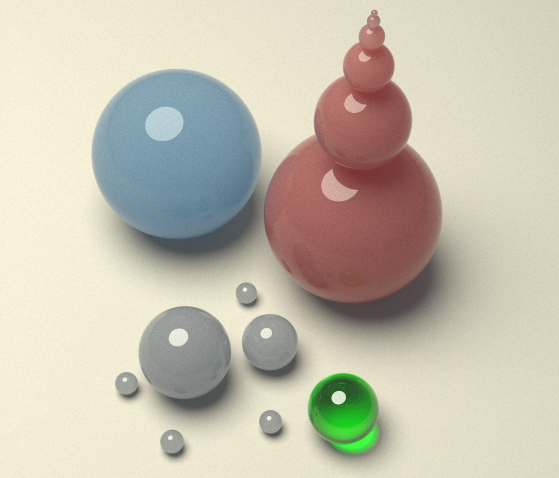
\includegraphics[width=0.9\linewidth]{./images/sss.png}}\label{sss}
    \caption{Example of subsurface scattering}
\end{figure}

\subsubsection{Global illumination}

Pathtracing allows to render images of three-dimensional scenes such that the global illumination is faithful to reality. Pathtracing naturally simulates many effects such as \textbf{soft shadows}, \textbf{ambient occlusion}, \textbf{color bleeding}, \textbf{caustics}, \ldots

\subsubsection{Implementation}
For implementation details about all the above effects, see the fully-commented file \textit{radiance.glsl}.

\section{SFX}

\subsubsection{Depth of field}

Depth of field can be easily integrated by "integrating" over the lens aperture and defining a focal distance. \\
See \textit{dof.glsl} for implementation details.\\

ADD PICTURES


\subsubsection{Antialiasing}

By casting several jittered ray per pixel to gather multiple samples, antialiasing comes in as a by-product.

\subsubsection{Tone mapping}

In order to have visually pleasing and realistic images, I applied a tonemap operator to scale the computed intensities while keeping the image constrast. I used tonemap operator used in the game \textit{Uncharted 2}.\\
See \textit{tonemap.glsl} for implementation details.


\section{Scenes}

The scenes use a sky background and sun (see \textit{sunsky.glsl}). \\
The sun constitutes a direct light source, while the sky contributes as a indirect one.


\section{Limitations \& further improvements}

In its current state, the pathtracer lacks a good UI to tweak the scene parameters. For now, every is coded is the shaders but these shaders can be modified at runtime and automatically reload. \\
The pathtracer also lacks the support of 3D models and easy scene configurations.\\
Another improvement would be the implementation of a bidirectional pathtracer in order to be able the produce caustics and light reflection in mirrors while keeping a good speed. \\
Finally, the code pathtracer can be further optimized by reducing the branching in the GLSL code and by profiling it.

\end{document}
